The proposed control structure is tested in the AAU Smart Water Infrastructure Lab (SWIL). This modular laboratory consists of a number of units pumping units (PU), consumer units (CU), and piping units (PiU) that can be used for small-scale emulation of a real WDN.

\begin{figure}[h!]
	\includegraphics[width=\linewidth]{Pictures/SWIL.pdf}
	\caption{Picture of the AAU SWIL}
	\label{fig:AAUSWIL}
\end{figure}

The network topology in \cref{fig:ImplementedWDN} is emulated via two PUs, a CU with two adjustable one-way valves each emulating a consumer, and a CU with an open bidirectional valve acting as the EWR, interconnected via two PiUs. Geodesic heights are emulated by pressuring the CUs. Experiments run for $12$ hours, with consumer demand curves based on real data and compressed to a fundamental frequency of $4$ hours such that each experiment corresponds to $3$ days. The controller attempts to follow a constant level reference throughout, starting $15 \si{mm}$ beneath it. After $4$ hours, a system leakage is simulated by fully opening the consumer valves for $30$ seconds. After $8$ hours, $50\%$ packet loss is introduced in the outer loop, which operates on a simulated TOD protocol. The tank level is seen on \cref{fig:OuterLoop}, while a snapshot of pump behaviour is seen on \cref{fig:InnerLoop}. The disturbance estimation scheme and true consumer flows can be seen on \cref{fig:DisturbanceEstimation}, with a zoomed-in view around the leakage seen on \cref{fig:Leakage}.

\clearpage

\begin{figure}[h!]
	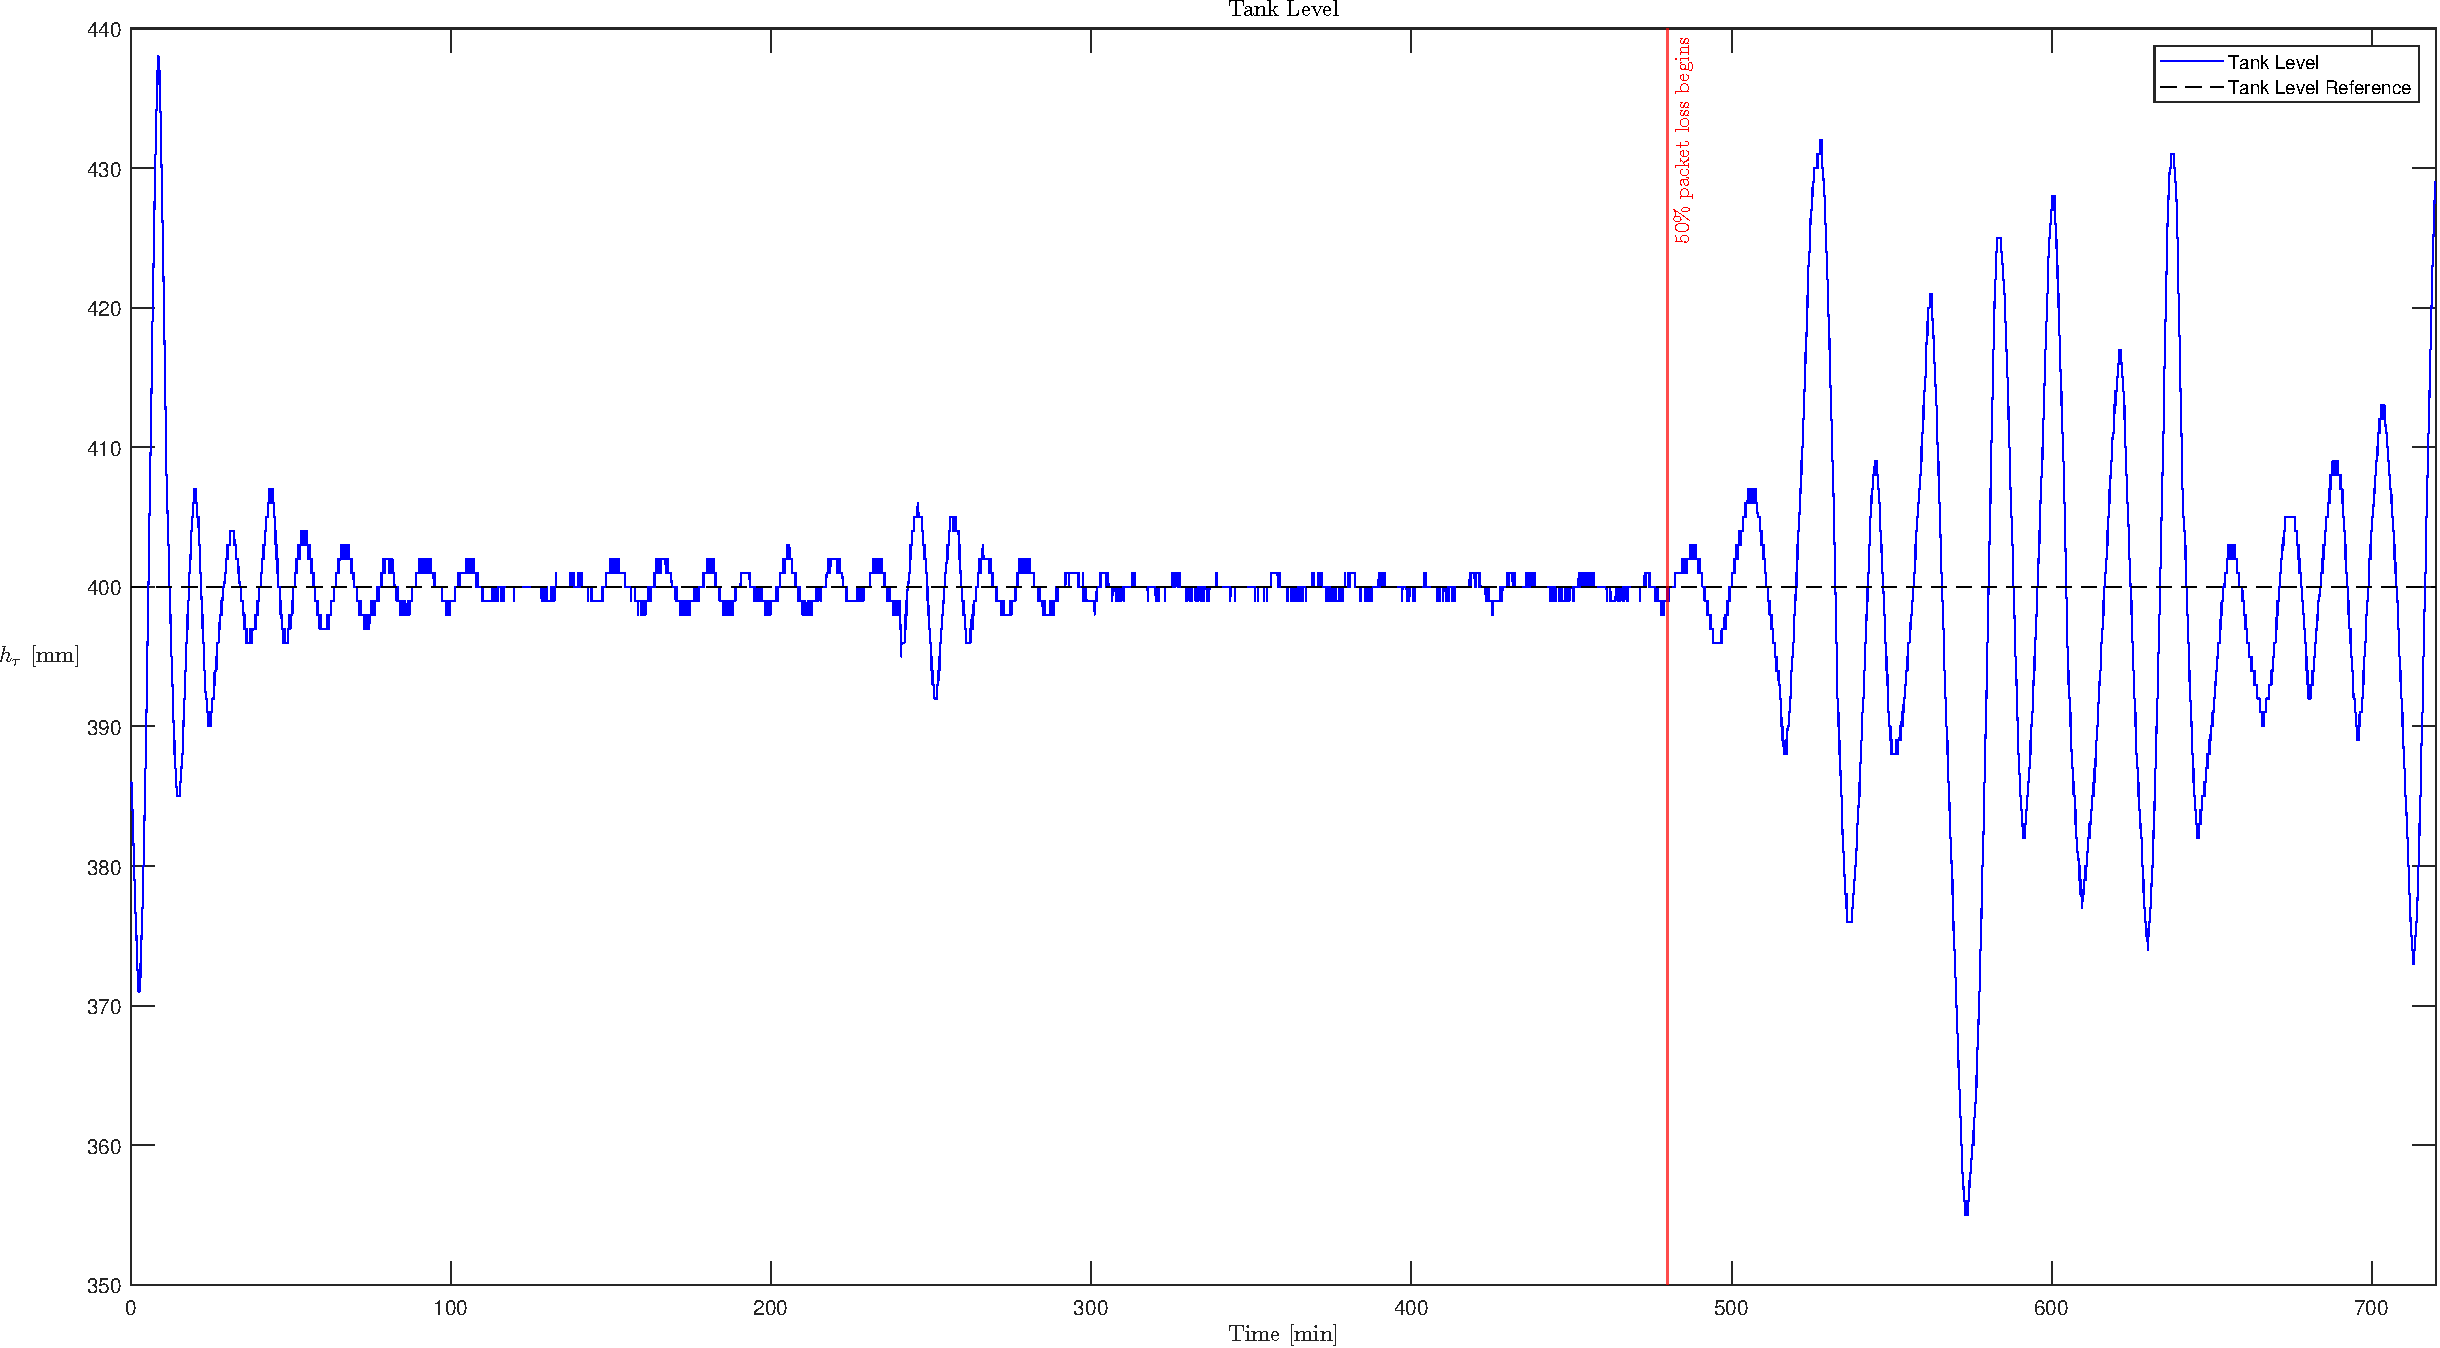
\includegraphics[height=8cm,width=\linewidth]{Pictures/OuterLoop.pdf}
	\caption{Outer loop controller performance.}
	\label{fig:OuterLoop}
\end{figure}

\begin{figure}[h!]
	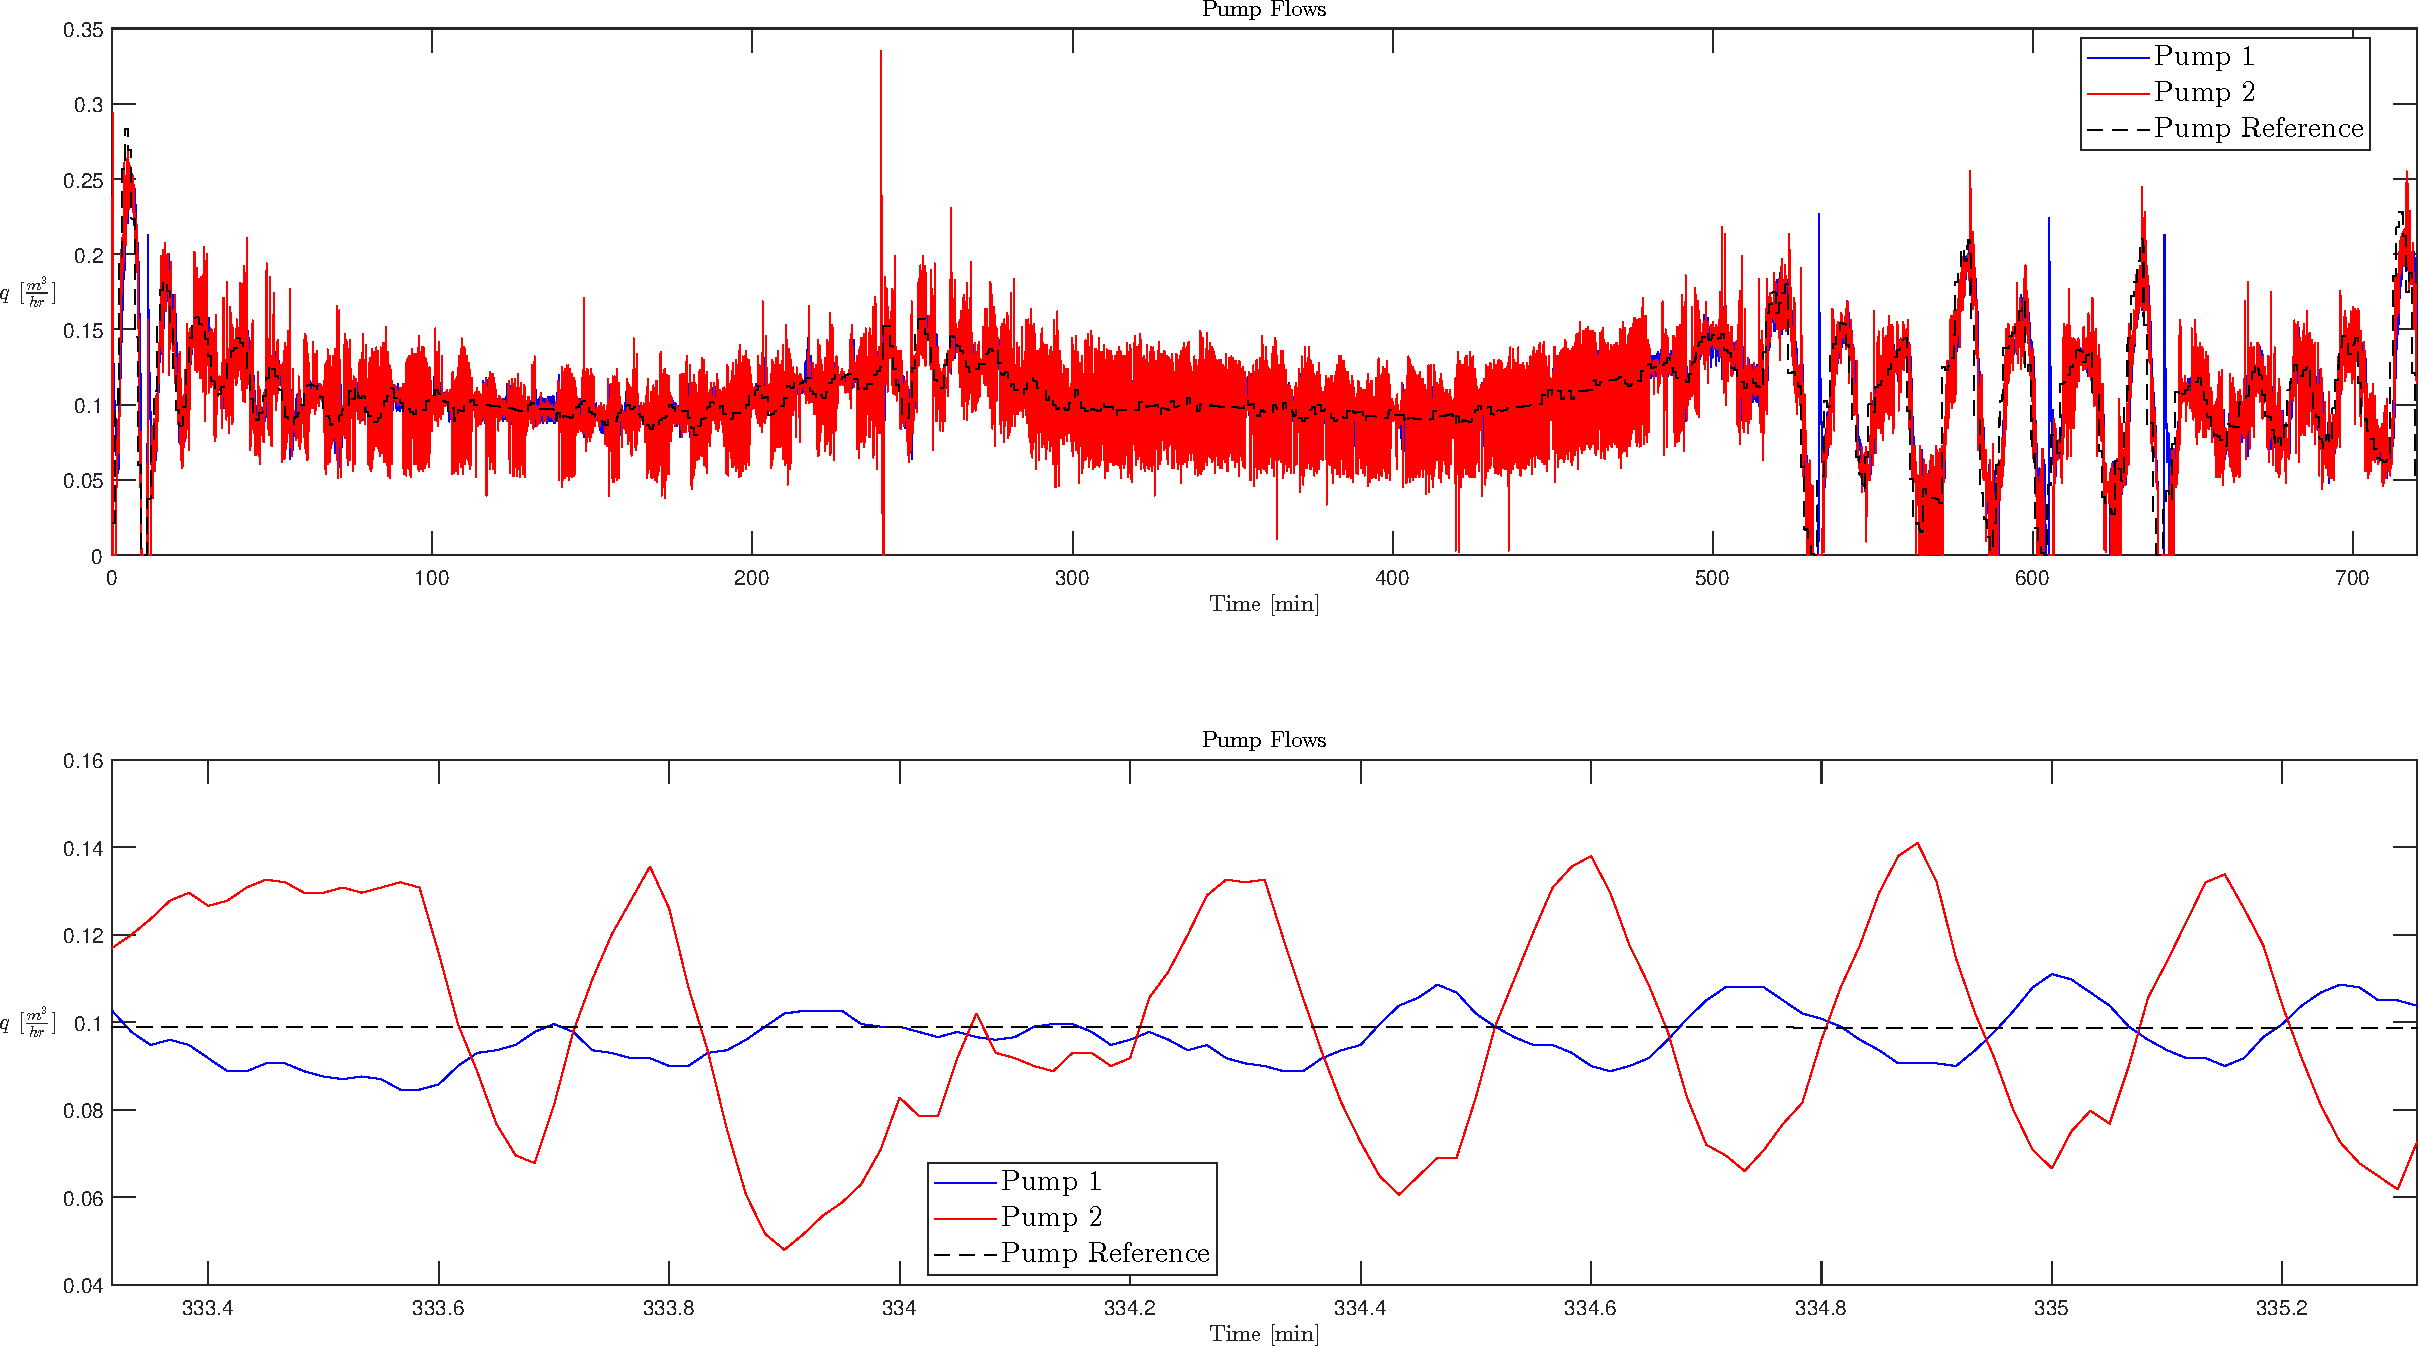
\includegraphics[height=8cm,width=\linewidth]{Pictures/InnerLoop.pdf}
	\caption{Inner loop controller performance.}
	\label{fig:InnerLoop}
\end{figure}

\begin{figure}[h!]
	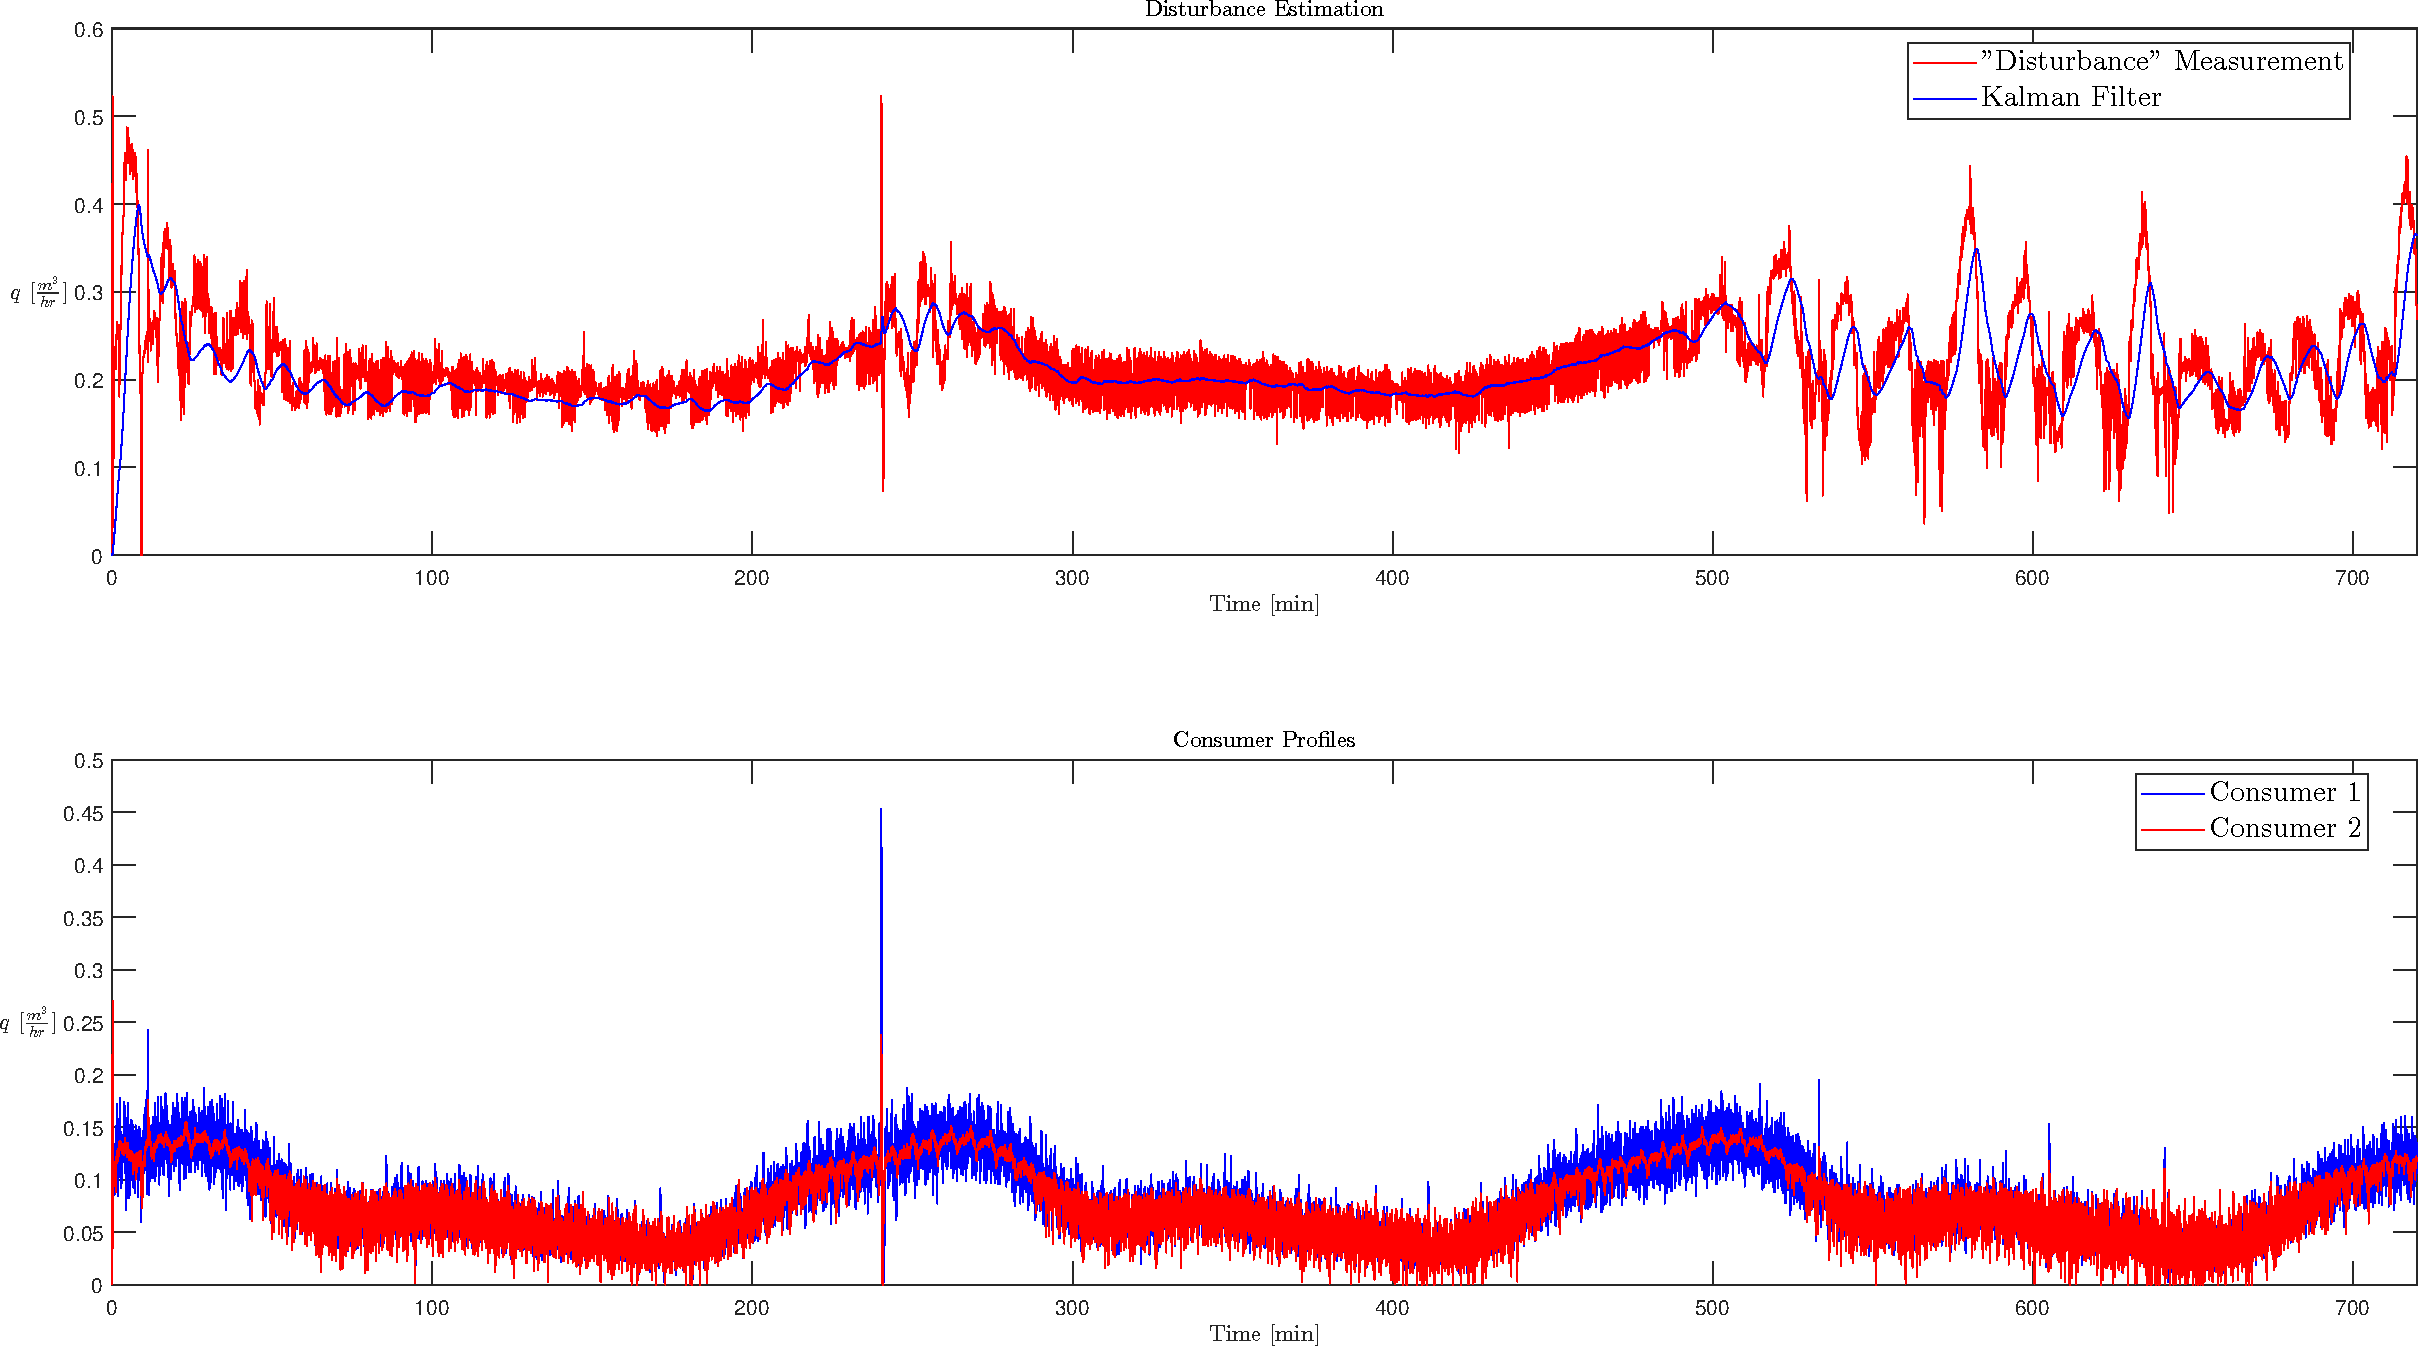
\includegraphics[height=8cm,width=\linewidth]{Pictures/DisturbanceEstimation.pdf}
	\caption{Kalman filter performance and consumer disturbances.}
	\label{fig:DisturbanceEstimation}
\end{figure}

\begin{figure}[h!]
	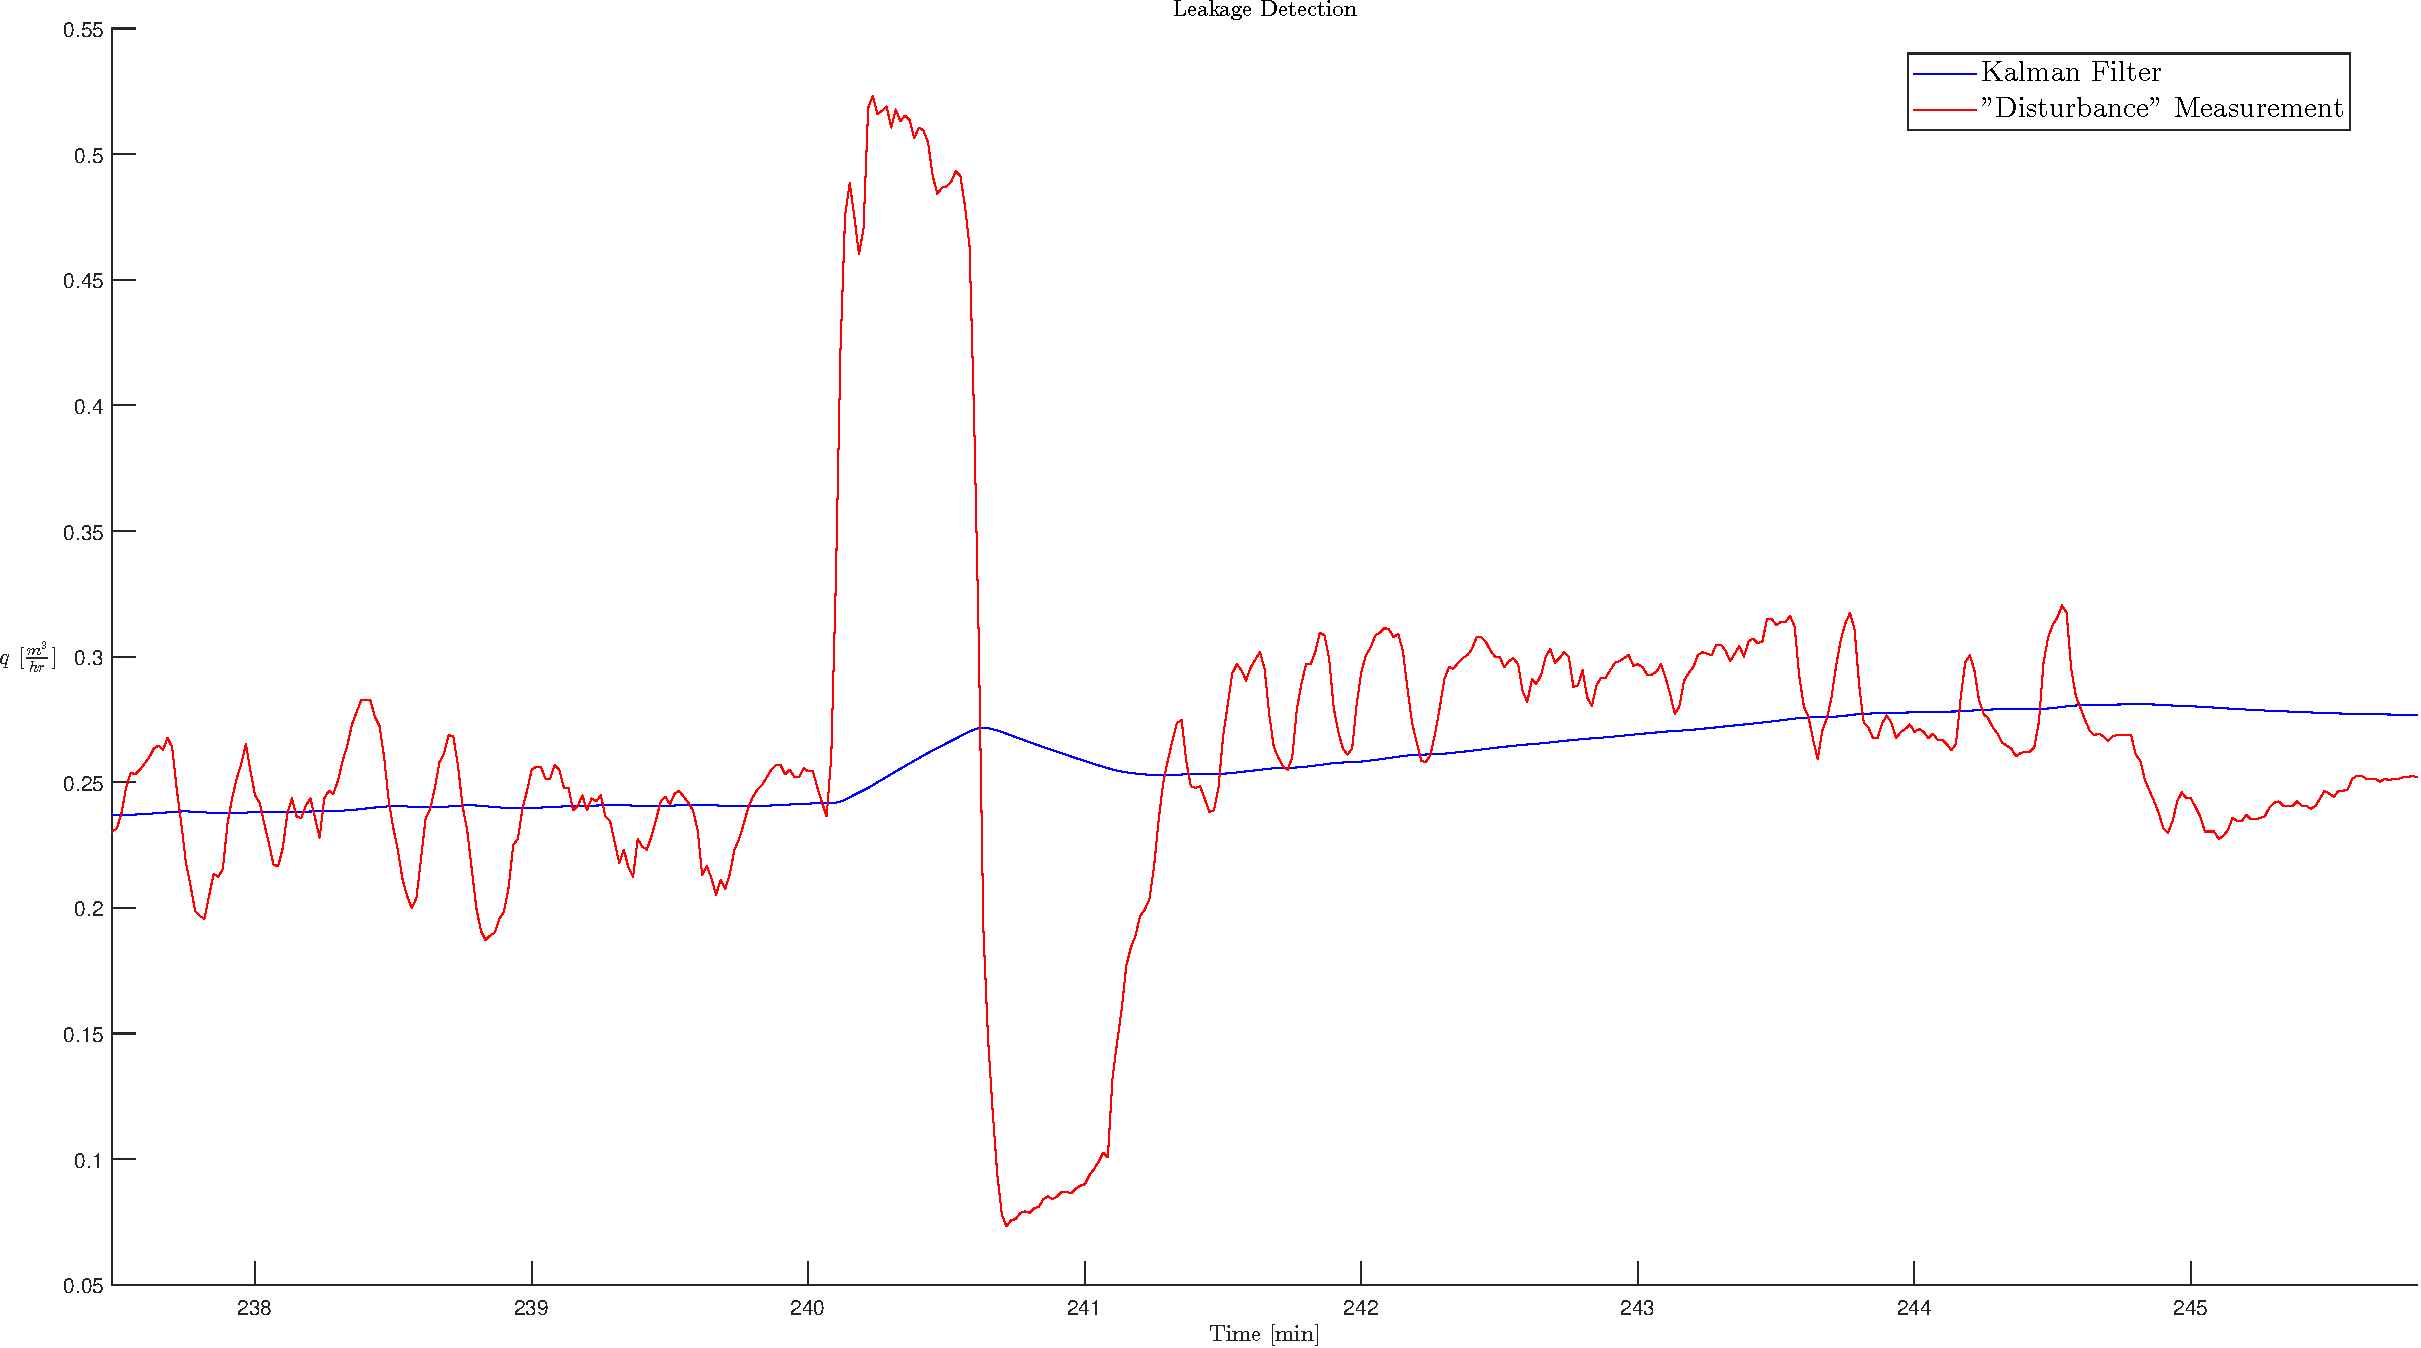
\includegraphics[height=8cm,width=\linewidth]{Pictures/LeakageDetection.pdf}
	\caption{Kalman filter-based leakage detection.}
	\label{fig:Leakage}
\end{figure}

It can be seen on \cref{fig:OuterLoop} that the outer loop eventually settles to within the quantisation error of the level sensor, i.e. tracks with zero measurable offset. It remains at this level for several hours, until $50\%$ packet loss is introduced after $8$ hours. A small transient is seen at $4$ hours, induced by the leakage, from which the system recovers with little issue. We note on \cref{fig:Leakage} that it is clearly possible to catch this leakage based evaluation of the residual between measurement and the Kalman filter. 

We note furthermore that the system clearly cannot converge to the reference and remain there for an extended period until the Kalman filter has converged to roughly the trajectory of the true consumer disturbance. This is mostly clearly seen by the difference between the short period from $\approx \{120 \ldots 160 \} \ \si{min}$, and the longer period from $\approx 300 \ \si{min}$ until packet loss is introduced: 

\clearpage

\begin{itemize}
	\item In the former case, the system reaches the reference level and remains there for some period of time. However, inspecting the Kalman filter on \cref{fig:DisturbanceEstimation}, it is clear that this has yet to settle to the true disturbance trajectory, and still exhibits significant oscillations. These oscillations eventually drive the outer loop away from the reference again.
	\item In the latter case, the Kalman filter has converged to approximately the true trajectory of the consumer-induced disturbance. Per \cref{fig:InnerLoop} the pump reference trajectory induced by the VF-LQR controller tracks it approximately, rather than oscillating as in the former case.
\end{itemize}  

Interestingly, this performance is possible despite the fact that it is largely impossible to achieve the exact reference specified in the inner loop. Charitably, the pumps tend to achieve the reference in a mean-square sense, but as evidenced by \cref{fig:InnerLoop}, the pumps have very clear cross-coupling that is somehow not reflected in the linearised model, and it is no surprise that two SISO controllers with no decoupling strategy cannot achieve the desired controller performance in this case, but instead give rise to a periodic steady-state solution. We note additionally that the model derived from first-principles is quite inaccurate; PI controller parameters had to be adjusted upwards by a factor of around $4$ via manual tuning in the lab. Controller performance in the inner loop is further hindered by the frankly \textit{dreadful} state of the SWIL flow sensors; these have a deadband of almost $0.1 \si{\frac{m^3}{hr}}$, and thus PI controllers working solely of their measurements cannot actually drive the flows in the system to $0$. To compensate for this serious sensor deficiency, we instead implemented forced $0$-clamping of the pump speeds whenever the reference delivered by the VFR-LQR is $0$, with an accompanying complete reset of the PI integrator terms. While this solves the sensor issue, it obviously comes at cost to the performance of the controller.

Tuning of the outer loop is similarly difficult in practice. The primary issue arises from the coupling between the outer loop and the Kalman filter, which is induced by the use of the measurement $\hat{d}_c = d_p - d_\tau$. This coupling means that transients in the outer loop are mapped into the Kalman filter, and vice-versa. Commensurately, these must be tuned extremely carefully to achieve the kind of performance seen in \cref{fig:OuterLoop}. Specifically, estimator transients induced by the controller must fall outside the passband of the Kalman filter, while the controller transients induced by the estimation error must either be insignificant or fall outside the bandwidth of the controller. A clear example of this can be seen on \cref{fig:OuterLoopBad,fig:DisturbanceEstimationBad}.

\clearpage

\begin{figure}[h!]
	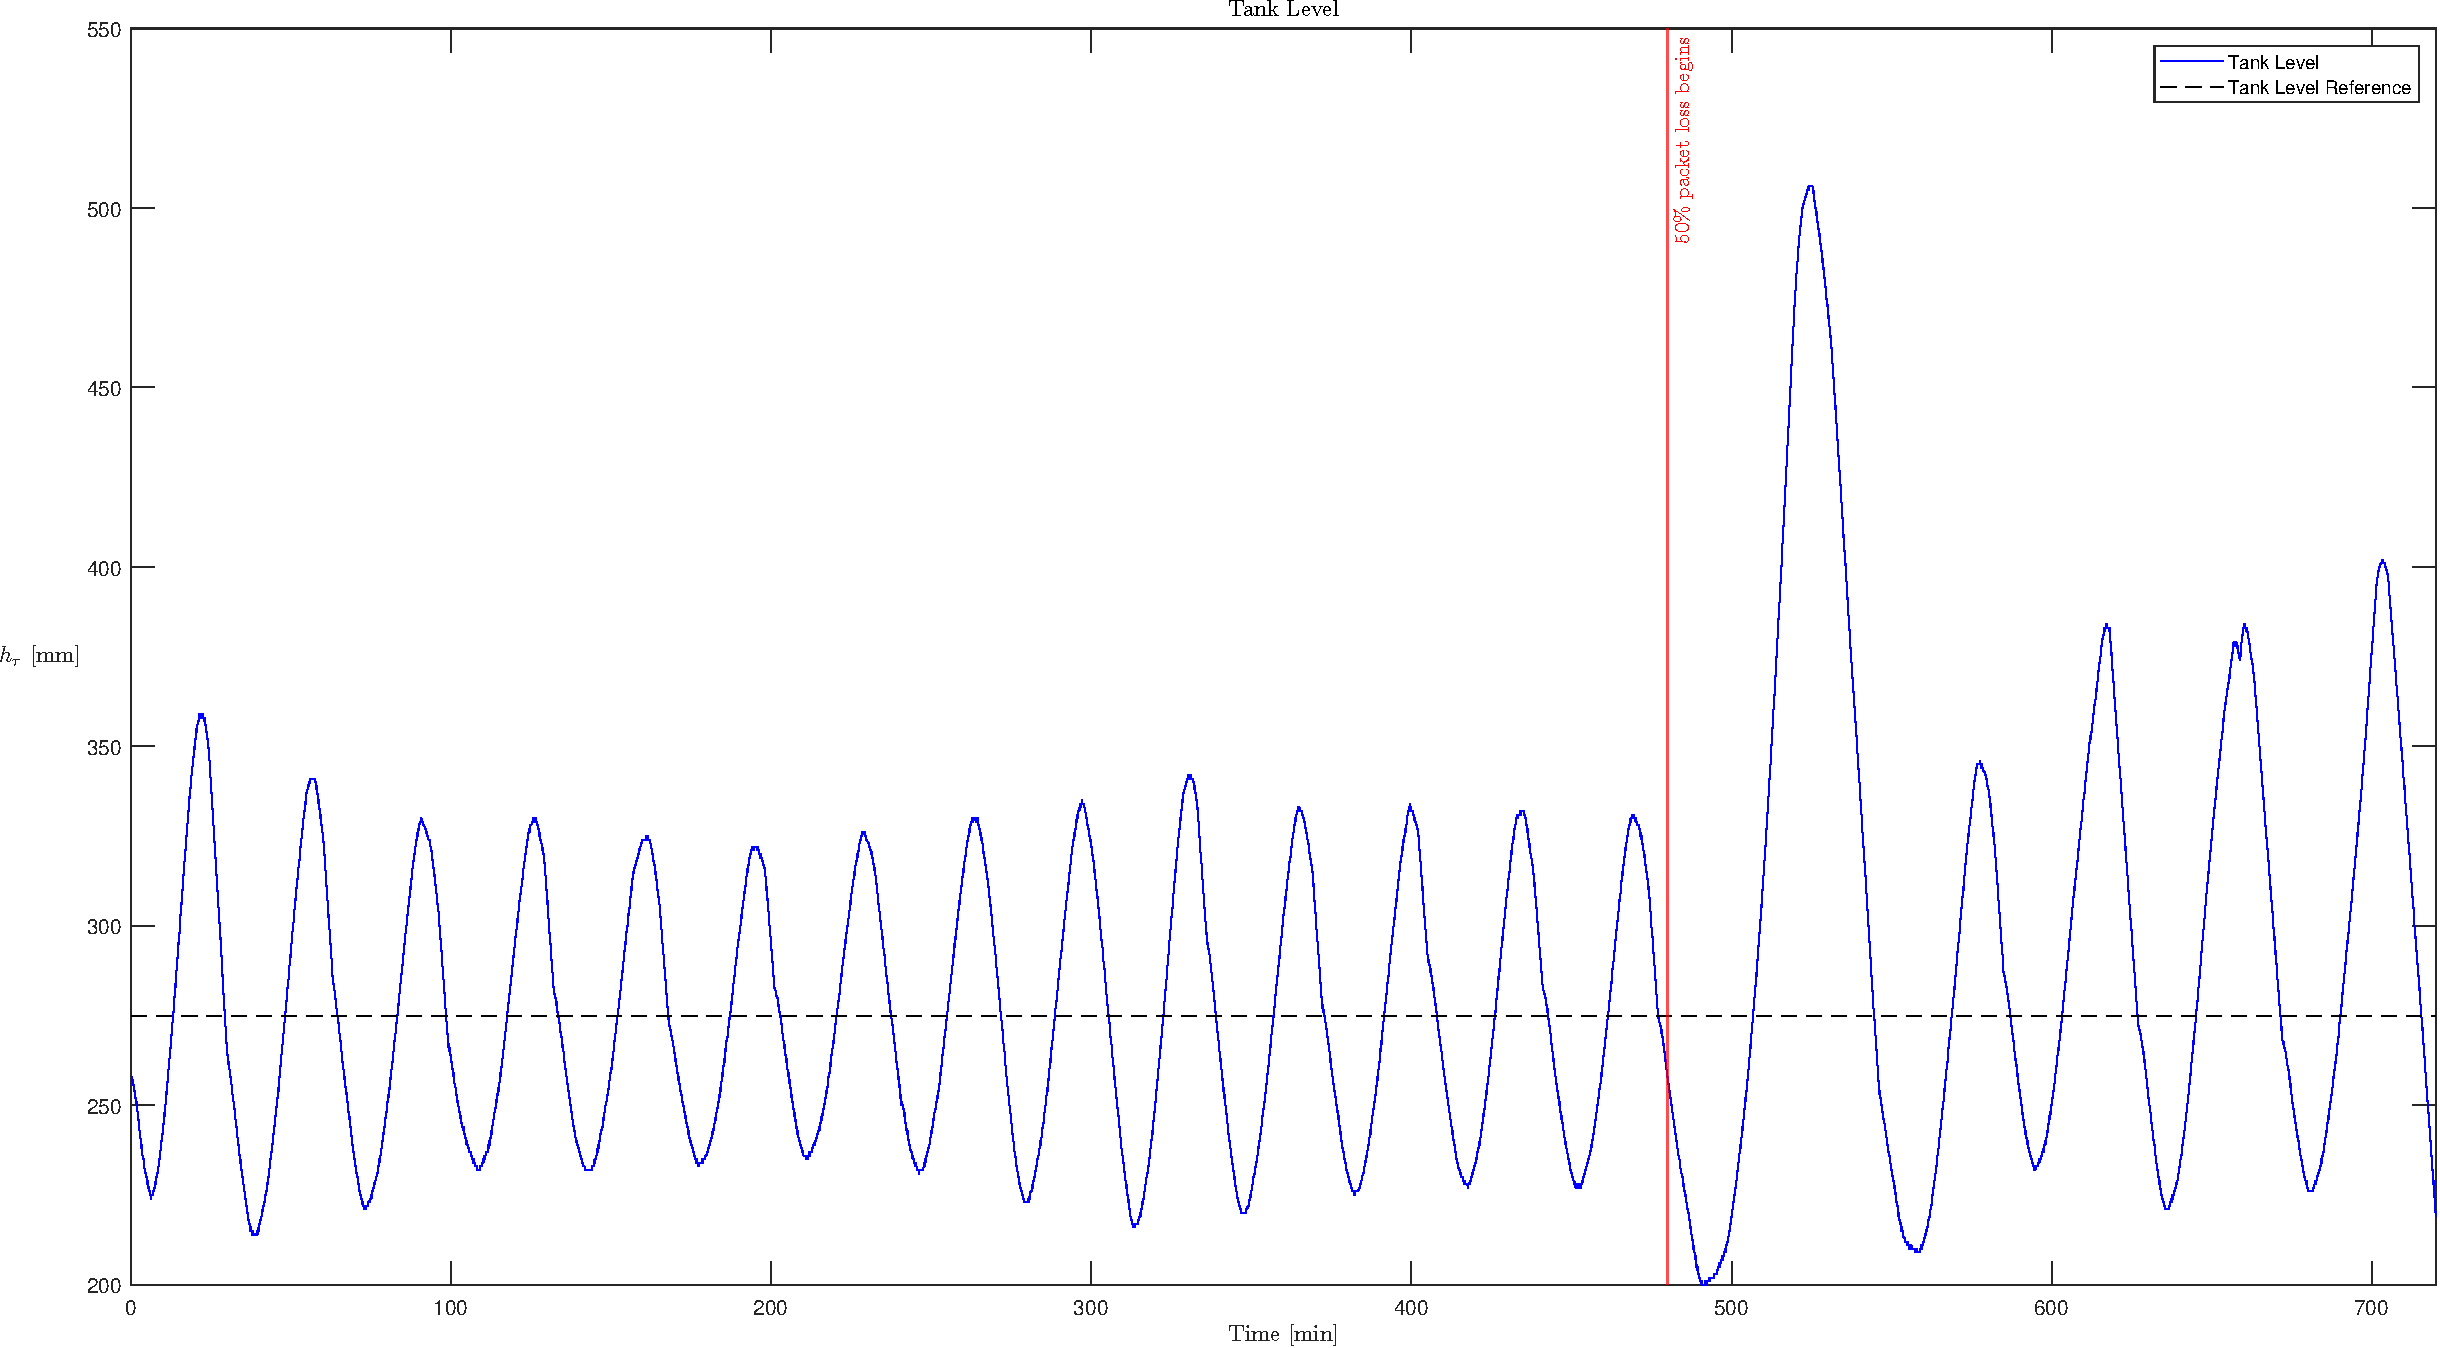
\includegraphics[height=8cm,width=\linewidth]{Pictures/OuterLoopBad.pdf}
	\caption{Outer loop controller performance, poor tuning.}
	\label{fig:OuterLoopBad}
\end{figure}

\begin{figure}[h!]
	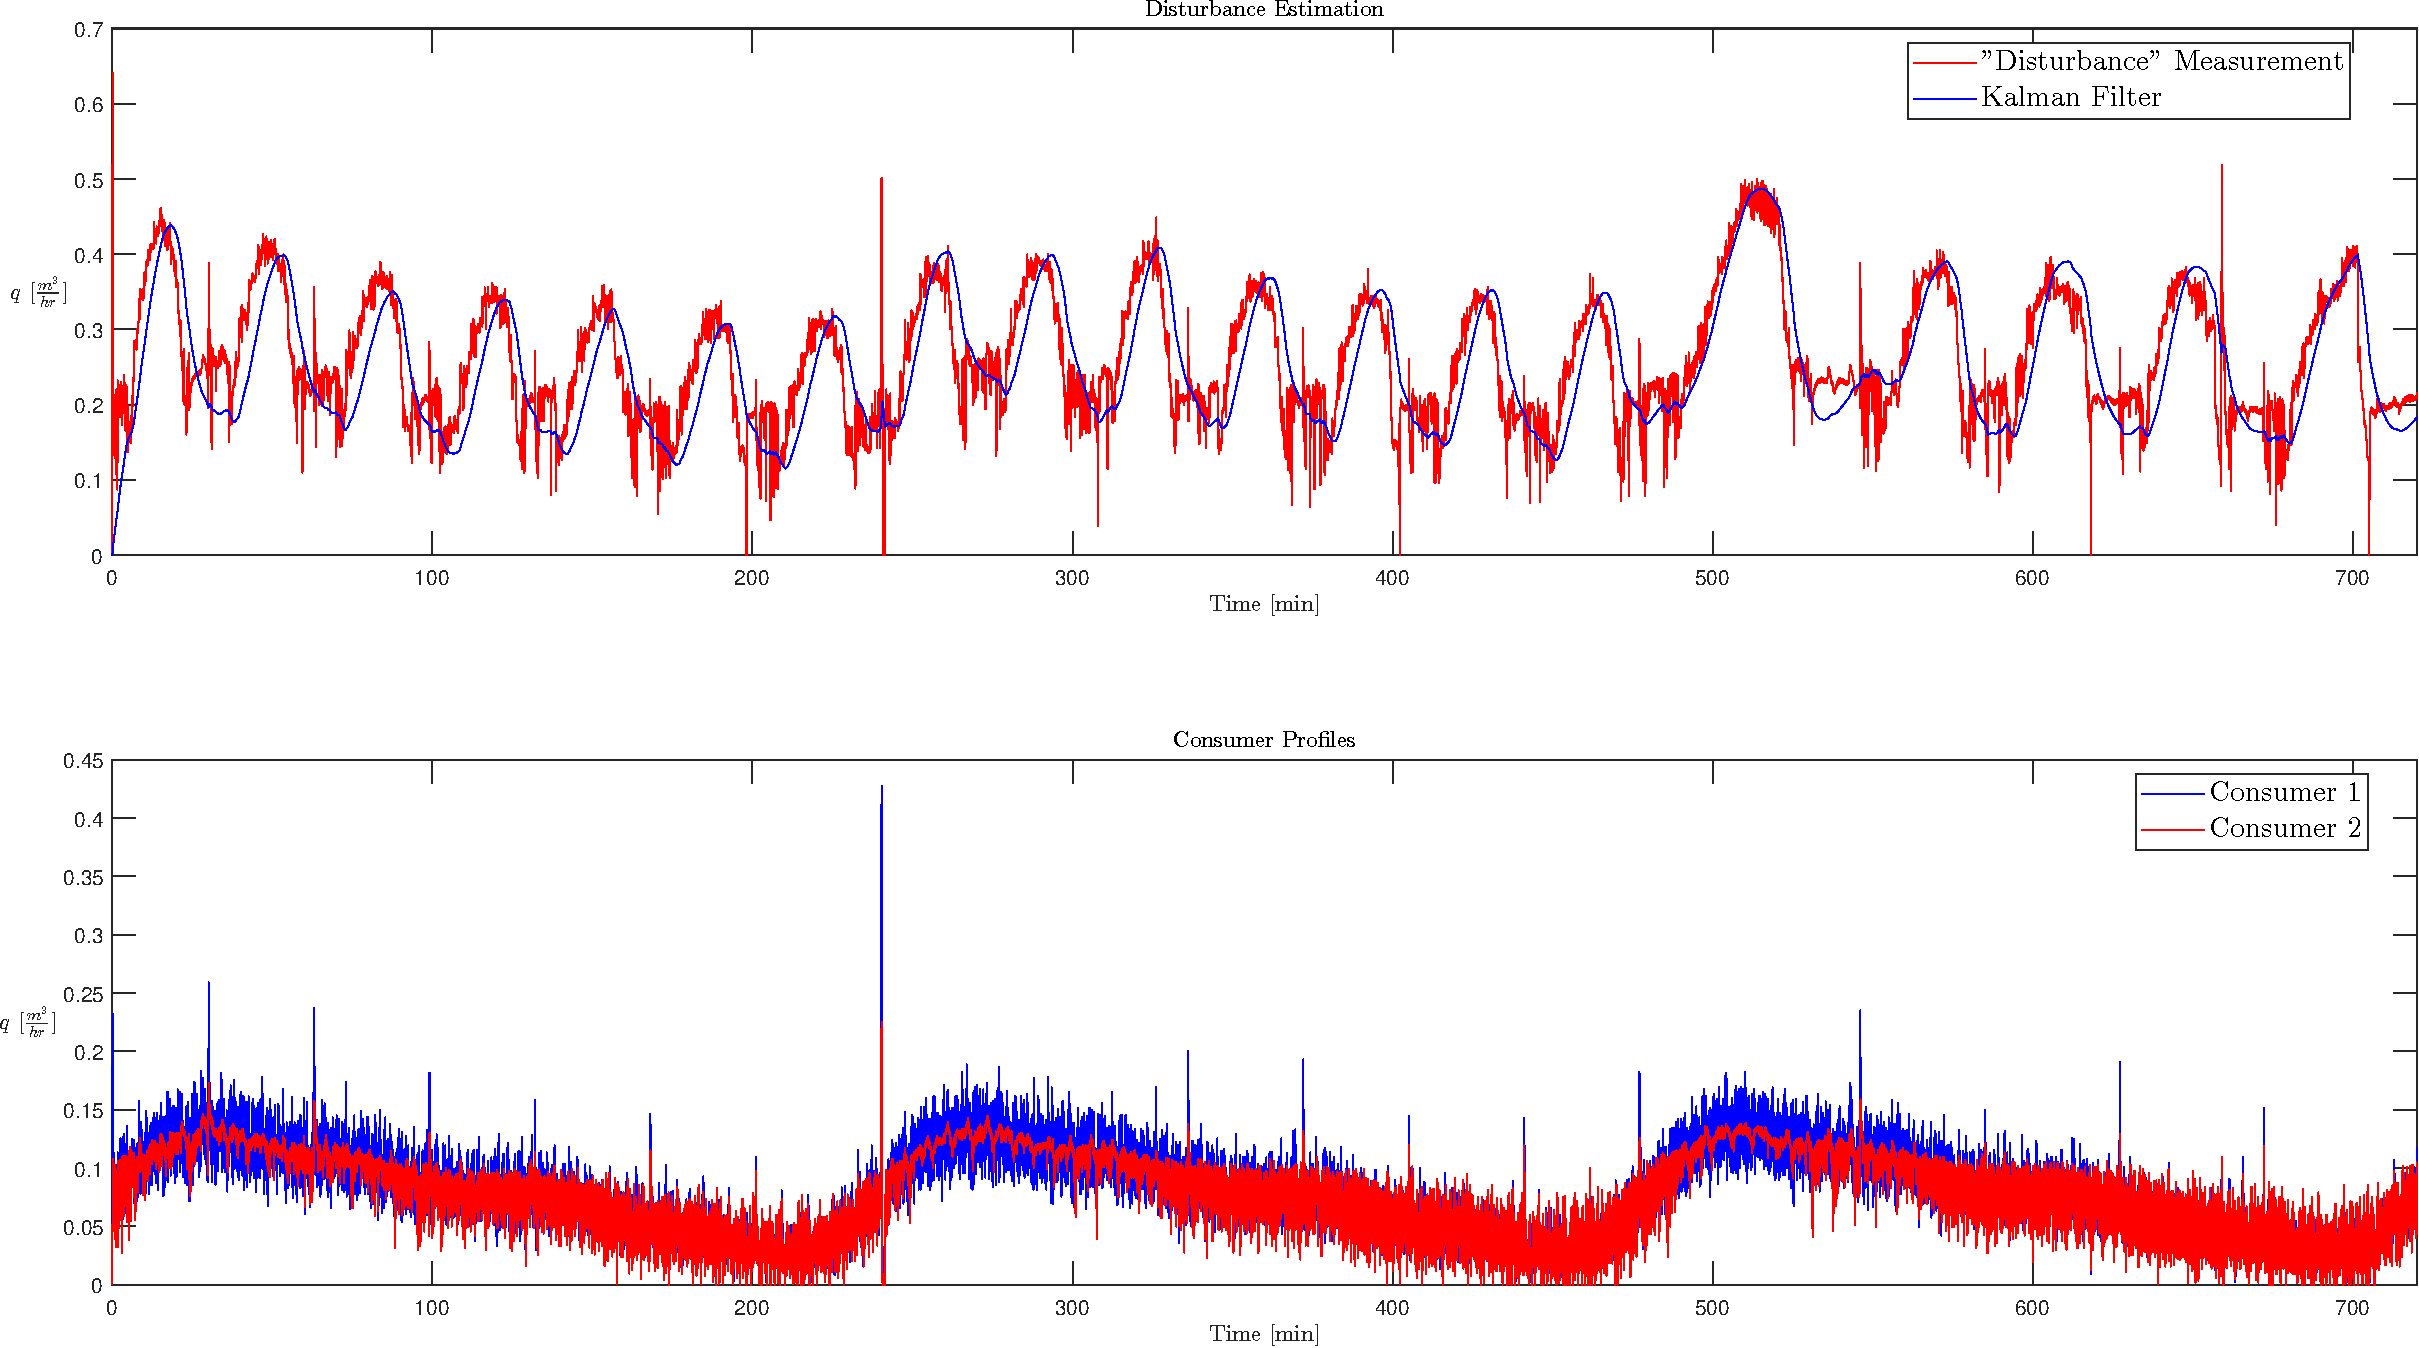
\includegraphics[height=8cm,width=\linewidth]{Pictures/DisturbanceEstimationBad.pdf}
	\caption{Kalman filter performance and consumer disturbances, poor tuning.}
	\label{fig:DisturbanceEstimationBad}
\end{figure}

We see that in this case, the controller and estimator mutually perturb each other, leading to performance that arguably resembles a pair of coupled oscillators. This is unfortunately a quite common result of the proposed control strategy; performance as in \cref{fig:OuterLoop} is very much confined to a small "Goldilocks" zone, at least for the given consumer disturbance profiles and size of the tank. We note, however, that the tank in this system is very small compared to what might be expected of a real-world WDN EWR, and therefore it is not unreasonable to consider these results close to worst-case conditions.